\chapter{Netwerken}

\section{Maken van een WIFI access point}\label{sec:AccesPoint}
	\paragraph{Probleem:} Je wilt een privé netwerk creëren door het bordje te gebruiken als WIFI access point.
	
	\paragraph{Oplossing:}
	\lstinputlisting{code/WIFI_AccessPoint.py}
	\paragraph{Discussie:} De Metro M4 Express heeft een tweede processor op het bordje, de ESP32. De ESP32 heeft WIFI en de coprocessor wordt gebruikt om het netwerk en communicatie over het netwerk te regelen. De ESP32 kan niet direct geprogrammeerd worden en het instellen en communiceren met de coprocessor gebeurt via SPI communicatie. De details hiervan zijn onbelangrijk, omdat Adafruit een bibliotheek heeft die deze communicatie regelt. Je hoeft dus alleen te weten hoe je gebruik maakt van deze bibliotheek. Zorg ervoor dat de adafruit\_esp32spi bibliotheek up to date is en in de lib folder staat op je bordje, zie hoofdstuk~\ref{sec:library}.
	
	Als je gebruik wilt maken van de ESP32 zijn altijd dezelfde 5 regels code nodig om controle te krijgen over de ESP32. Deze stappen zijn te zien onder de comment "setup ESP32 control". De laatste stap cre\"eert een esp object met een heleboel mogelijkheden voor het gebruik van het netwerk. \'E\'en daarvan is het opzetten van een access point. De create\_AP() methode heeft als eerste parameter de naam van het netwerk en als tweede parameter het password. "Pass" in de while loop zorgt dat de loop niks doet, maar het programma wel blijft draaien. Als het programma klaar is wordt het netwerk namelijk gelijk weer afgebroken. Als alles goed gegaan is, staat de naam van je gecreëerde netwerk tussen je WIFI netwerken, zoals in Figuur~\ref{fig:AccessPoint}. Als je inlogt op dit netwerk heb je geen toegang meer tot het internet, omdat dit een priv\'e netwerk is.
	
	\begin{figure}[!htb]
		\center{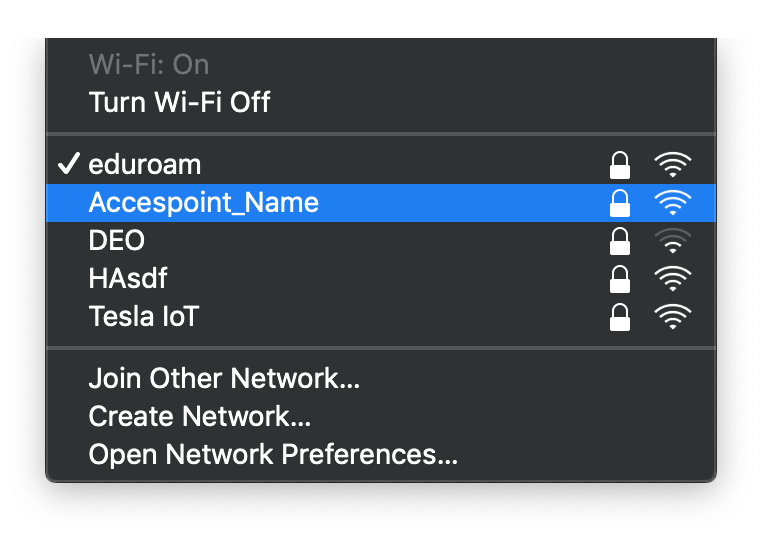
\includegraphics[width=0.6\linewidth]{figures/AccessPoint.png}}
		\caption{Access point in WIFI netwerken}
		\label{fig:AccessPoint}
	\end{figure}
	
	\paragraph{Meer informatie}\textbf{:}\\
	\url{https://circuitpython.readthedocs.io/projects/esp32spi/en/latest/api.html}


\section{Data sturen van client naar server over WIFI}\label{sec:WIFIdata}
	\paragraph{Probleem:} Je wilt over het WIFI netwerk data sturen naar het bordje en dit vervolgens printen naar de terminal.
	
	\subsection{Server}
		\paragraph{Probleem:} Je moet data kunnen ontvangen op je bordje via WIFI.
		\paragraph{Oplossing}: 
		\lstinputlisting{code/Minimal_Server.py}
		\paragraph{Discussie:} De code lijkt op het eerste gezicht heel complex en om het helemaal goed te begrijpen heb je kennis nodig over netwerk communicatie. Dat gaat dit project te buiten. Gelukkig is de code goed te gebruiken zonder al die kennis en is een globaal idee goed genoeg. 
		
		Om data uit te wisselen tussen het bordje en een ander apparaat zijn 2 dingen nodig. Ten eerste moeten de apparaten op hetzelfde netwerk zitten, dit wordt gedaan door met het bordje een priv\'e netwerk te cre\"eren en als access point te functioneren, zoals in ~\ref{sec:AccesPoint}. Ten tweede moet over dit netwerk een verbinding gemaakt worden tussen de twee apparaten, waarover ze informatie kunnen versturen. Let goed op dat er een verschil is tussen een netwerk en een verbinding. Heel het "world wide web"(internet) zit op hetzelfde netwerk, maar je hebt met je computer niet met alle websites een verbinding. 
		
		Achter de schermen draait een website op een \textit{server}. Een server is een computer dat een programma draait dat wacht tot een ander apparaat, een \textit{client}, een verbinding maakt. De client stuurt dan een datapakketje naar de server, waarin naar de gewenste pagina wordt gevraagd. De server ontvangt dit datapkketje, leest de aanvraag en stuurt de gewenste pagina terug naar de client.
		
		Dit principe wordt ook gebruikt voor het communiceren tussen je bordje en je computer. Eerst wordt een in de code een WIFI netwerk gecre\"eerd. Daarna wordt een server gestart op de esp32 met de adafruit\_esp32spi bibliotheek. Deze server wacht tot een client verbinding maakt. Dan gaat de code naar de oneindige while loop die uit 2 stukken bestaat. Het 1e stuk bevat nog een while loop, waar de code blijft loopen tot een client verbinding maakt. Als er dan een verbinding is gaat het door naar het 2e stuk met de if/elif statement. Er wordt gekeken of er een verbinding is en of er data is gestuurd door de client. Als dat het geval is wordt de data gedecodeerd en geprint naar de terminal. De plaats waar de print statement staat is de plek waar je ook andere dingen kan doen met de data, zoals motors aansturen en data terugsturen(zie recept~\ref{sec:RCservo}). Zolang de verbinding bestaat worden het eerste stuk met de while loop en het stuk met de elif statement overgeslagen en wordt alleen de if statement uitgevoerd als er data is verstuurd door de client. Anders gebeurt er niks en blijft het loopen tot er wel iets is gestuurd of de verbinding wordt verbroken. Als de client de verbinding verbreekt wordt de elif statement uitgevoerd en komt de code terug in de while loop, waar het programma wacht op een nieuwe verbinding.


\newpage
\subsection{Client}
	\paragraph{Probleem:} Je wilt data sturen naar een server vanaf je pc.
	\paragraph{Oplossing:}
	\lstinputlisting{code/Minimal_Client.py}
	\paragraph{Discussie:} De \textbf{client} kant moet niet ge\"upload worden op je bordje, maar moet je runnen met python op je computer. Houd er rekening mee dat de code alleen werkt als je op hetzelfde netwerk zit als je bordje. Log dus eerst in op het WIFI netwerk van je bordje.
	
	Verbinding maken met- en data sturen naar een server kan eenvoudig met de socket module van Python's standaard bibliotheek. Je geeft de server's host adres en port nummer en met 3 regels code kan je verbinden met de server. 
	
	In de oneidige while loop wordt de gebruiker gevraagd om een bericht te typen. Als dit bericht '-q' is wordt het programma afgesloten en anders wordt het geconverteerd naar een bytearray dat kan worden verstuurd met de sendall() methode van de socket library. Als het goed is zie je de text die je stuurt verschijnen in de REPL van Mu editor.
	


\section{Besturen van een servo met laptop}\label{sec:RCservo}
\paragraph{Probleem:} Je wilt over WIFI een servo aansturen.
\newpage
\subsection{Server}
\lstinputlisting{code/RC_Servo.py}

\subsection{Client}
\lstinputlisting{code/RC_Servo_Client.py}

\paragraph{Discussie:} Dit is een combinatie van het sturen van data over WIFI in recept~\ref{sec:WIFIdata} en het aansturen van een servo in recept~\ref{sec:servo}. Het enige verschil aan de \textit{Client} kant ten opzichte van recept~\ref{sec:WIFIdata} is dat je een hoek moet invoeren. Aan de server kant is het verschil dat de servo geinitialiseerd wordt en dat in plaats van data te printen, nu de hoek van de servo ingesteld wordt. 

\section{Gebruiken van keyboard toetsaanslagen}
\paragraph{Probleem:} Je wilt in een programma het keyboard van je laptop gebruiken.
\paragraph{Oplossing:}
\lstinputlisting{code/PrintKeyStroke.py}
\paragraph{Discussie:} Voor het gebruik van je keyboard heb je de python bibliotheek "keyboard" nodig. Open de terminal op je laptop en type: \newline
\\
pip install keyboard\\
\\
In de code wordt eerst de bibliotheek keyboard ge\"importeerd. Daarna wordt de functie gedefinieerd die bepaald wat er gebeurd als je een toets indrukt. Met keyboard.hook(functienaam) koppel je het keyboard aan de functie en 'luistert' het programma op de achtergrond naar toetsaanslagen. Bij een keyboard event, zoals het indrukken of loslaten van een toets, wordt de lopende code onderbroken en wordt een eventobject doorgegeven aan de functie. Het eventobject heeft de eigenschappen "name" en "event\_type". De name eigenschap is de toets en event\_type zegt of de toets is ingedrukt of losgelaten. In de oneindige while loop hoeft verder niks geprogrammeerd te worden, omdat door keyboard.hook() op de achtergrond geluisterd wordt. Het zou kunnen dat je de code als administrator moet runnen. Als de code werkt, worden de toetsnaam en toetsrichting naar de terminal geprint.
\\
\url{https://pypi.org/project/keyboard/}

\newpage
\section{Gebruik van keyboard om een Servo aan te sturen over WIFI}
\paragraph{Probleem:} Je wilt over WIFI met je keyboard een servo aansturen.

\paragraph{Benodigdheden:}
\begin{itemize}
	\item 1x Servo
\end{itemize}

\begin{figure}[H]
	\center{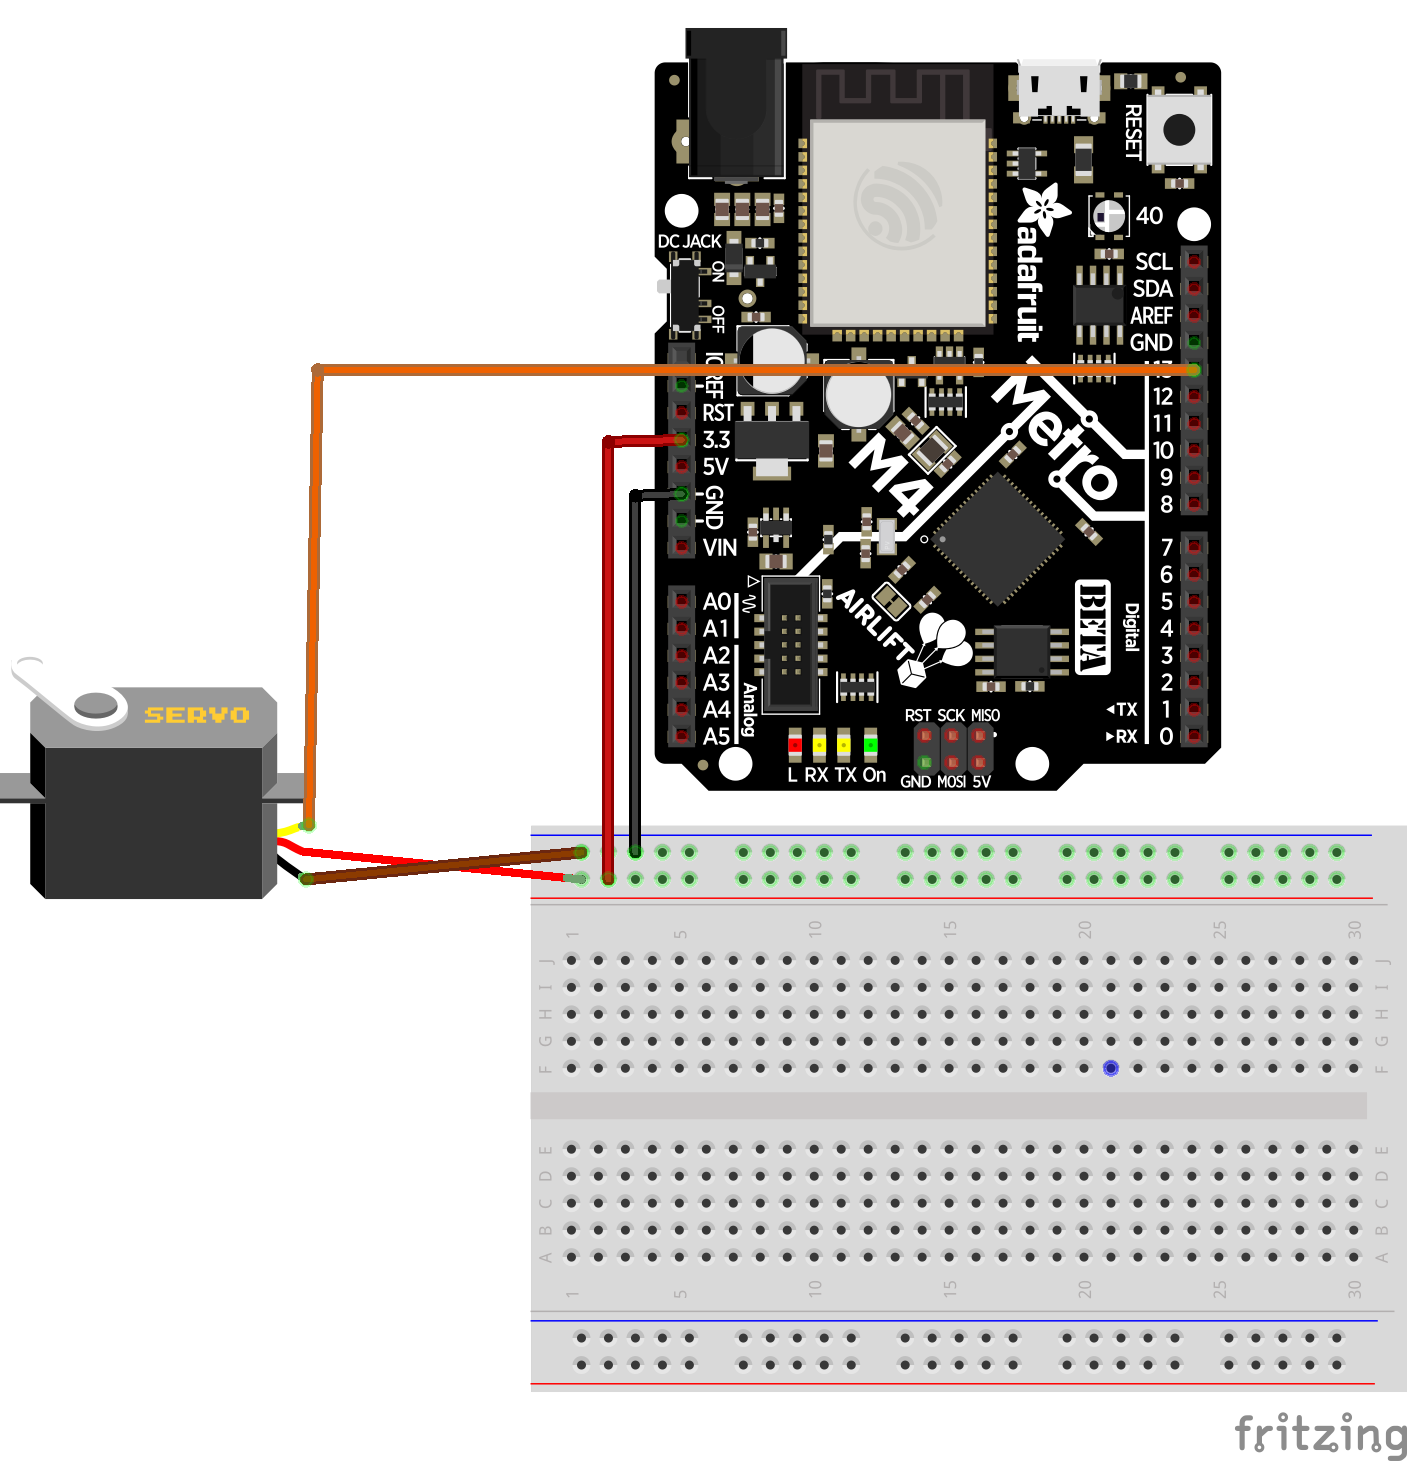
\includegraphics[width=0.6\linewidth]{figures/Servo.png}}
	\caption{Servo Circuit}
	\label{fig:ServoKeyboard}
\end{figure}


\subsection{Client:}\label{sub:KeyboardServoClient}
\paragraph{Oplossing:}
\lstinputlisting{code/Keyboard_Servo_Client_v2.py}


\paragraph{Discussie:} Om een servo met een keyboard te besturen over WIFI moeten 2 dingen gebeuren. Ten eerste moet bijgehouden worden welke knoppen zijn ingedrukt en ten tweede moet deze informatie over het netwerk gestuurd worden.\\\\

Laten we eerst kijken naar het bijhouden van welke knoppen zijn ingedrukt. Een dictionary met de naam button\_state wordt ge\"initialiseerd met de keys 'left' en 'right' om dit bij te houden. Om te zien hoe de dictionary gebruikt wordt, moeten je kijken naar de 3 functies om key events te regelen. De key\_handler() functie is de functie die met keyboard.hook() gebonden wordt aan het keyboard. Bij elk keyboard event wordt het programma onderbroken en wordt key\_handler() gerund. De key\_handler() functie kijkt dan of een knop is ingedrukt of losgelaten en stuurt het key\_event dan door naar de key\_press\_handler() functie als een knop is ingedrukt en naar de key\_release\_handler() als een knop is losgelaten. Deze functies kijken vervolgens om welke knop het gaat en zet in de button\_state dictionary een 1 als de knop is ingedrukt en een 0 als een knop is losgelaten. \\

Om deze informatie te sturen over het netwerk moet eerst een netwerk connectie gemaakt worden. Het maken van een netwerk en het sturen van data is al besproken in ~\ref{sec:WIFIdata} en ~\ref{sec:RCservo}. De data moet nog wel in een goede vorm gezet worden, zodat het over het netwerk gestuurd kan worden. Dit wordt gedaan in de infinite while loop. Eerst wordt de knoprichting bepaald van button\_state. Als alleen rechts is ingedrukt krijgt keyDirection de waarde 1, als alleen links is ingedrukt -1, als rechts en links zijn ingedrukt 0 en als niks is ingedrukt ook 0. \\

Voordat keyDirection over het netwerk gestuurd wordt, wordt gekeken of de richting anders is dan de laatst gestuurde waarde. Alleen als de waarde is veranderd wordt de nieuwe waarde over het netwerk gestuurd. Dit wordt gedaan om het netwerk te ontlasten. Het controleren van de verandering is de taak van de checkStateChange() functie, waar keyDirection vergeleken wordt met current\_direction en een 0 of 1 terug geeft als de richting respectievelijk niet of wel is veranderd. Als de richting is veranderd gaat het programma de if statement in. Eerst wordt de waarde met de sendData() functie gestuurd. In deze functie wordt keyDirection eerst verandert in een alfabetische letter met het gebruik van de PACK\_DICT. De waarden op deze manier "coderen" maakt het een stuk eenvoudiger om de data na het sturen weer uit te pakken. 
Data wordt namelijk byte voor byte verzonden. \'E\'en string character is gelijk aan 1 byte. Als je de waarde -1 converteert naar de string '-1' moeten 2 bytes verstuurd worden, de - en de 1. Deze variabele lengte maakt waarden uitpakken aan de kant van de ontvanger een stuk complexer, mede doordat meerdere waarden in de buffer kunnen staan. De waarden 0,1,0,-1,0,-1 uit de string "010-10-1" vereist meer dan alleen splitsen, omdat er soms 1 en soms 2 characters gebruikt worden voor een waarde. "bcbaba" splitsen in b,c,b,a,b,a en vervolgens omzetten met een dictionary in 0,1,0,-1,0,-1 maakt dit heel eenvoudig. 
Na het coderen van de waarden in de sendData() functie, wordt de character met .encode() verandert in binaire data en vervolgens verstuurd met sendall().
Tot slot wordt current\_direction ge\"updatet en wacht het programma \SI{50}{\milli\second} voordat het opnieuw de while loop doorloopt. 


\newpage
\subsection{Server}\label{sub:KeyboardServoServer}
\paragraph{Oplossing:}
\lstinputlisting{code/Keyboard_Servo_Server_v2.py}


\paragraph{Discussie:} De server kant is voor het grootste deel te vergelijken met \ref{sec:RCservo}. Het grootste verschil is wat voor data er binnen komt en hoe hier mee omgegaan wordt. De data wordt uitgelezen in de oneindige while loop met de recv() methode. We verwachten hier van de client kant een gecodeerde character of een string met characters, afhankelijk van hoeveel er gestuurd zijn en in de buffer staan. We zijn alleen ge\"interesseerd in de laatste character, omdat deze de recentste toestand weergeeft en moeten deze destilleren van de buffer. De bytearray wordt eerst geconverteerd naar een string en vervolgens wordt de laatste character uit de string gehaald. Deze alfabetische letter wordt gedecodeerd met de UNPACK\_DICT. UNPACK\_DICT is een soort van de omgekeerde PACK\_DICT, alleen wordt a,b,c nu omgezet in de servo waarden 0, 90, 180, in plaats van de toetswaarden -1,0,1. Na het destilleren van de laatst gestuurde waarde kan gelijk de servo ingesteld worden.\\


